\begin{wrapfigure}[0]{r}[9pt]{0cm}
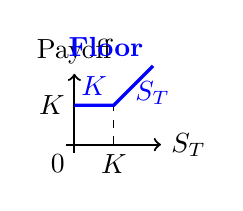
\begin{tikzpicture}[scale=1]
    % --- 定义坐标和参数 ---
    % K 代表执行价格的位置，调整为0.5以适应0-1的范围
    \def\K{0.5}
    % 定义图表的延伸范围，已根据要求修改为1
    \def\maxST{1}
    \def\maxPayoff{0.8}

    % --- 绘制坐标轴 ---
    % 坐标轴稍微延伸出定义范围一点点，留出箭头空间
    \draw[->, thick] (-0.1, 0) -- (\maxST + 0.1, 0) node[right] {$S_T$};
    \draw[->, thick] (0, -0.1) -- (0, \maxPayoff + 0.1) node[above] {Payoff};

    % --- 绘制辅助线和标签 (Strike K) ---
    % 在x轴上标记 K
    \draw[dashed, thin] (\K, 0) node[below] {$K$} -- (\K, \K);
    % 在y轴上标记 K (Floor level)
    \draw[dashed, thin] (0, \K) node[left] {$K$} -- (\K, \K);
    % 标记原点
    \node[below left] at (0,0) {0};

    % --- 绘制组成部分 (虚线) ---
    % 由于空间变小，去掉了过于冗长的文字标签，保留核心线条以便参照
    % 1. Long Asset Payoff (Payoff = S_T)
    %\draw[gray, dashed, thick] (0, 0) -- (\maxST, \maxST);

    % 2. Long Put Option Payoff (Payoff = max(K - S_T, 0))
    %\draw[gray, dashed, thick] (0, \K) -- (\K, 0) -- (\maxST, 0);

    % --- 绘制最终的 Floor Payoff (实线粗线) ---
    % Floor Payoff = max(K, S_T)
    \draw[blue, very thick] (0, \K) -- (\K, \K) -- (\maxST, \maxST);

    % --- 添加简化的标签 ---
    % 调整了标签位置和大小以适应紧凑的空间
    % 水平段的 Payoff = K
    \node[blue, above] at (\K/2, \K) {$K$};
    % 斜线段的 Payoff = S_T
    \node[blue, right] at (\K+0.15, \K+0.15) {$S_T$};
    % 总标签
    \node[blue, anchor=south east] at (\maxST, \maxST) {\textbf{Floor}};

\end{tikzpicture}
 \end{wrapfigure}